\chapter{Programmable Logic Controllers (PLCs)}
\begin{quotation}
    \textsf{\textbf{Introduction} TO DO...}
\end{quotation}
\minitoc

\begin{figure}[h]
    \centering
    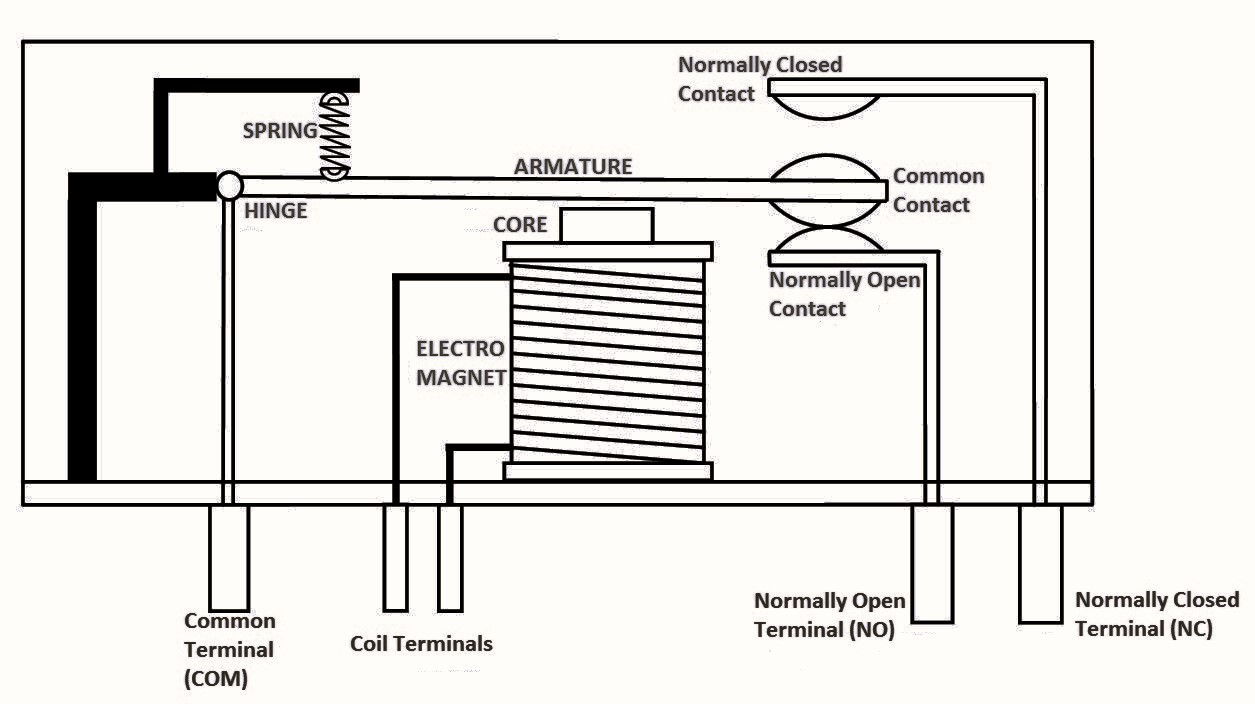
\includegraphics[scale=0.4]{img/relay_scheme.jpg}
    \caption{Relay scheme }    
\end{figure}
\vspace{-0.5cm}
\section{Industrial Automation Hardware}
In the field of \textit{Industrial automation} the controllere can be found at different places: (i) directly in the senso or in the actuator (analog PIDs), as a separate device or as an algorithm in a computer (here there is the possibility to manage a great number of loops). There are many possibilities to realize a controller: 
\begin{description}
    \item[Wired relay systems] At first in absence of computers and programmable devices, controllers was realized through \textit{\textbf{relays}}\footnote{
        A \textbf{relay} is a simple electromechanical device that use a magnetic field to control a switch. In this device there is a coil that, when energized creates a magnetic field that pushing a piece of metal close/open the switch.
    } and dedicated control loops; the number of such devices for automating the production was not negligible: you can imagine that the changeover time was not short at all, too. The schematic given by the engineers to the electricians which embeds the logic to implement was called \textit{ladder schematic} which used to display sensors, motors, valves, relays you were able to find into the system. Such systems were based on mechanical systems whose moveable parts represented a problem to face. Moreover, if only one relay stopped working, the entire system had to be checked.
    \item[Analog circuits] A step forward was made introducing \textit{operational amplifier} in order to implement PID controllers; there are several circuits exploiting the \textit{virtual ground principle} in order to simulate the proportional, integrative and derivative blocks.   
    \item[Embedded circuits] More modern technologies which are \textit{microprocessor-based}. They are designed for a specific task and are parts of more complex systems including other hardware and mechanical parts. They have a lot of advantages, among the other: low power consumption and reduced sizes. They can be based on microcrocontroollers, DSP, microprocessors or FPGAs.
    \item[Industrial PC] It is nothing but a PC integrated with specific expansions, machine interfaces, expanded communication ports and so on. They are characterized by different construction properties which make them more suitable to the context they are used in (for example: alternative cooling methoeds, heavier metal for the external frame...)
    \item[PLCs] (Programmable Logic Controllers) whose main features are well-explained in the next paragraphs. 
\end{description}

\section{The advent of PLCs}
The realization of low cost computer made possible the most recent evolution in automatin industrial plants: the advent of PLCs. This phenomena begain in 70s. More specifically, in 1968 \textit{General Motors} issued a first PLC prototype request in order to progressively substitute hard-wired relays.
\begin{definition}
    A \textbf{PLC} is a real-time microprocessor-based system that implement functions as   \textit{logic, sequencing, timing} and \textit{arithmetic operations} in order to perform some control tasks.
\end{definition}

PLCs, probably, will remain predominant on the factory floor. This is due to some particular features:
\begin{itemize}
    \itemsep-0.3em
    \item They can be used to control complex mutlivariable systems; 
    \item They are reprogrammable, for this reason they can be reapplied to different systems; 
    \item The fact a computational abitily can be used, they can address even more complicated control tasks.
    \item They have analog and digital I/Os with standard levels. Depending on the tipology they can have a large number of peripherals.
    \item They are relatively cheap, while the value is the in the application software.
\end{itemize}

\begin{figure}
    \centering
    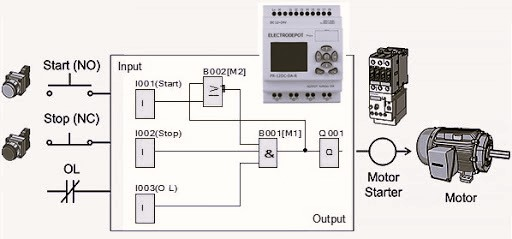
\includegraphics[scale=0.7]{img/PLC_scheme.jpg}
    \caption{An example schematic for a PLC}
\end{figure}

The first PLCs were programmmed using the same schematic used for describing the realization of wired relay-based systems (ladder diagrams). This eliminated the need to teach the technicians to program them. Nowadays, ladder diagrams are the most common way to program a PLC. \\
It is remarkable, that there is a standard, the IEC 61131-3, which enumerates five programming languages for PLCs which are splittable into two categories: (i) \textbf{graphical languages} which comprises Function Block Diagram (FBD), Ladder Diagram (LD) and Sequential Flow Chart (SFC); (ii) \textbf{textual languages} which comprises Instruction List and Structured text.

\subsection{PLC connections}
How the PLCs is used? When a process is controlled by using a PLC it uses input from sensors to make decisions and provides outputs which drives actuators. The control loop, as usual, is continuous cycle for: (i) reading the  inputs, (ii) solving the ladder logic, (iii) changing the outputs accordingly.

\section{Ladder diagrams}  
How we mentioned before, \textbf{ladder logic} is the main programming method for PLCs that mimic the relay logic and it has been explained why the decision to use it was a strategic one\footnote{Note that nowadays relays are also used in modern control systems but not for implementing the logic which is almost totally demanded to PLCs}.
An example of ladder schematic is given in the \Cref{fig:ladder}.

\begin{figure}[h]
    \centering
    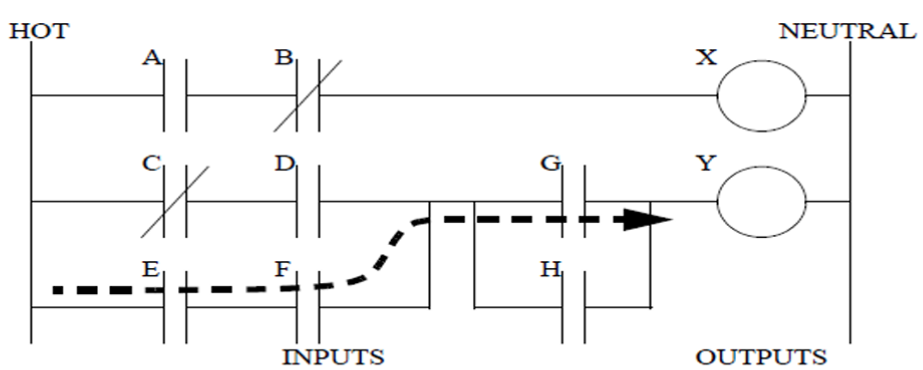
\includegraphics[scale=0.5]{img/sample.png}
    \caption{Example of ladder schematic}
    \label{fig:ladder}
\end{figure}

Just to give a bit of terminology, the power flows from left to  right among two rails which are called \textbf{hot} and \textbf{neutral} rails. A basic element of a ladder schematic is the \textbf{rung} which in which there are combinations of \textit{inputs} (vertical lines, barred vertical lines) and \textit{outputs} (circles). An input can come from a sensor, while the \textit{output} is some device which is external from the controller (light, motors) which is switched on or switched off.

\subsection{Ladder logic Inputs}

\subsection{Ladder logic Outputs}

\subsection{Example: Design of an alarm for an house}

\subsection{Latch, Counters, Timers}

\section{Examples on Ladder schematics}

\subsubsection{E1: Basic Logic Functions}

\subsubsection{Car Safety system}

\subsubsection{Motor Forward/Reverse}

\subsubsection{A Burglar alarm}


